\chapter{Fictitious Forces using Free Body Diagnrams}

The concept of Fictitious forces is something that should not be use in general practice to determine the required dynamics of the given problem statement. Fictitious forces are not actual forces, instead put in place so as to give meaning to accelerations that generate due to the dynamics of the problem while under a certain motion. For example, centrifugal (or centripetal) accelerations that are experienced by the a body under circular motion is given a meaning using the concept of fictitious forces as in a way this acceleration acts as a force in order to keep the dynamics of the problem stable under a certain motion. In this case, centripetal force (or centrifugal) force keeps the body stable while it is cornering (or going around circles). It is important to always remember that these fictitious forces do not exists in reality, however, the accelerations such as centripetal accelerations do appear from the type of geometry and dynamics of the system.

The meaning to such fictitious forces is given using free body diagrams. To understand this in more detail consider figure \ref{Fig_0_ch_3_fictitiousForces1} of a 1D rotation problem which is similar to the problem discussed in section \ref{Sec_TorqueAndAngularMomentumProblem2}. However, here the mass on the link is fixed firmly such that the motion along $\hat{r}$ direction is constrained as follows
\begin{equation}
	\dot{r} = \ddot{r} = 0
\end{equation}
further, the link is allowed to rotate in a variable rotational rate such that
\begin{align}
	\omega &= \dot{\theta} \hat{k} \\
	\dot{\omega} &= \ddot{\theta} \hat{k}
\end{align}
are allowed.
\newpage
\begin{figure}[h!]
	\centering
	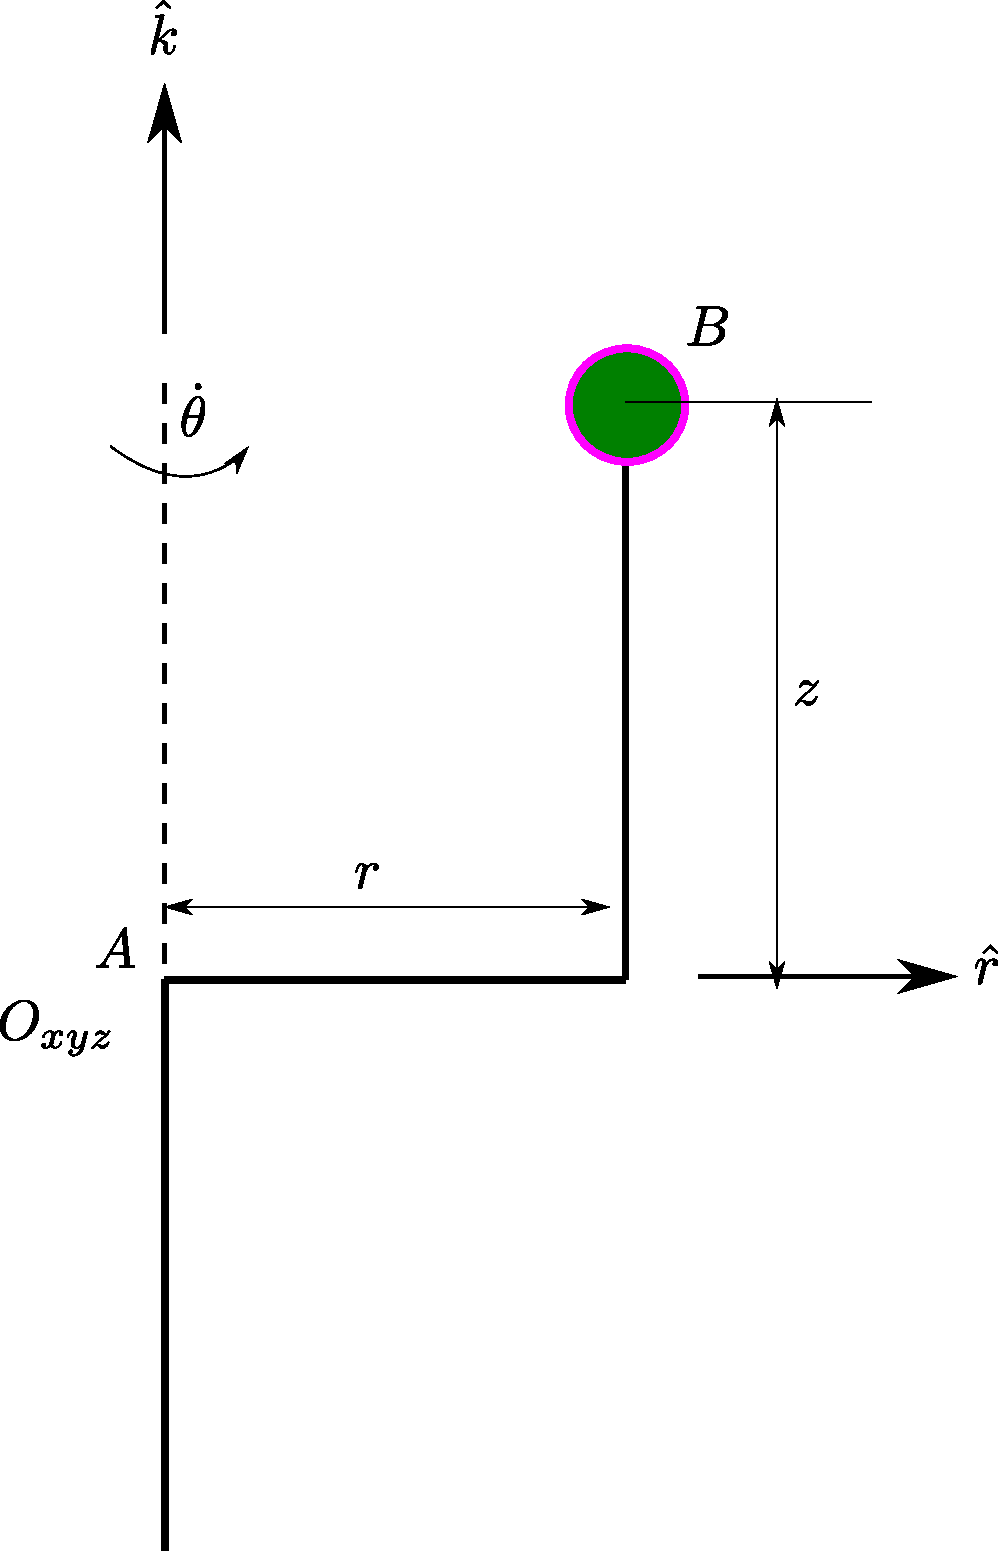
\includegraphics[width=0.5\linewidth]{Bilder/16_FictitiousForces1.pdf}
	\caption{Rotation problem to describe fictitious forces}
	\label{Fig_0_ch_3_fictitiousForces1}
\end{figure}
In order to find the accelerations on the system, consider equation \eqref{Eq_accelrationInPolarCoordinates}:
\begin{equation}
a_{B/O} = a_{A/O} + (\ddot{r}\hat{r} + \ddot{z}\hat{k}) + 2 \dot{r} \dot{\theta} \hat{\theta} +  r \ddot{\theta} \hat{\theta} - r \dot{\theta}^{2} \hat{r}
\end{equation}
here $a_{A/O} = 0$, $\ddot{r} = 0$, $\ddot{z} = 0$, therefore, reducing the above equation to:
\begin{equation}
a_{B/O} = r \ddot{\theta} \hat{\theta} - r \dot{\theta}^{2} \hat{r}
\end{equation}
using Newtons second law, the forces along $\hat{r}$ and $\hat{\theta}$ can be expressed as
\begin{align}
	\sum F_{r} &= - m r \dot{\theta}^{2} \hat{r} \label{Eq_0_ch_3_ff_1} \\
	\sum F_{\theta} &= m r \ddot{\theta} \hat{\theta}
\end{align}
clearly, the system is stable and it seems like that due to these accelerations there are forces acting on the mass $B$ such that these forces keep the mass stable under rotation, by keeping it in a stable circular motion. If we consider these accelerations to be labeled as forces, then we can use free body diagrams in order to explain and name them as some kind of force. Using the free body diagram as shown in figure \ref{Fig_0_ch_3_fictitiousForces1_1}
\newpage
\begin{figure}[h!]
	\centering
	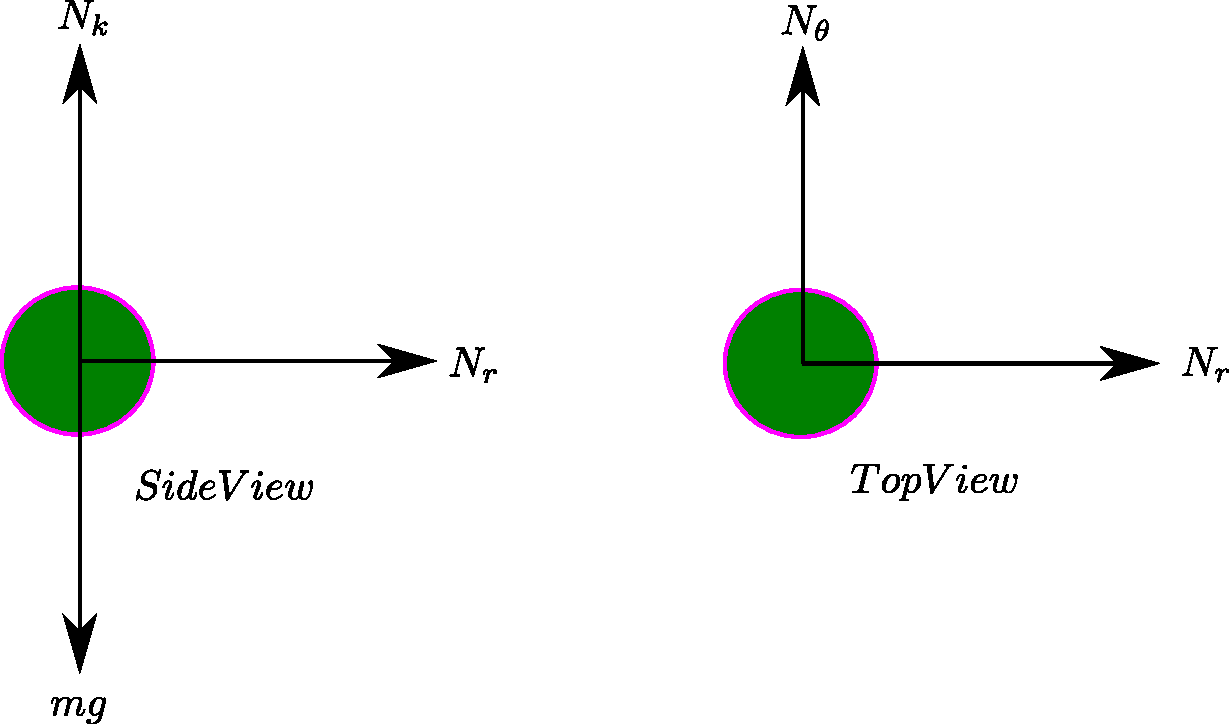
\includegraphics[width=0.7\linewidth]{Bilder/16_FictitiousForces1_1.pdf}
	\caption{Naming fictitious forces using FBD's}
	\label{Fig_0_ch_3_fictitiousForces1_1}
\end{figure}
Lets assume that the forces acting along the three polar coordinate directions are labeled as shown in figure \ref{Fig_0_ch_3_fictitiousForces1_1}, using the FBD and equation \eqref{Eq_0_ch_3_ff_1} it can be said that
\begin{equation}
	\sum F_{r} = N_{r} = - m r \dot{\theta}^{2} \hat{r}
\end{equation}
or that
\begin{equation}
\sum F_{r} = N_{r} + m r \dot{\theta}^{2} \hat{r} = 0
\end{equation}
which is true as  there are no external forces that are acting on the system along $\hat{r}$ direction. Note that using FBD, we considered that there is a force acting in the system $N_{r}$, which is not true as there is no force acting there. In essence, $N_{r} = 0$, so there is no force to cancel out the force due to centripetal acceleration $- r \dot{\theta}^{2} \hat{r}$. In other words, centripetal force $- m r \dot{\theta}^{2} \hat{r}$ exists only because we considered $N_r$ in the first place and we have multiplied mass to the centripetal acceleration $- r \dot{\theta}^{2} \hat{r}$ to treat it as a force instead of acceleration.

It is always confusing to explain the fictitious forces, only because they don't exists in reality. What exists is only the accelerations. In some physics problems (very few old ones), sometimes people use fictitious forces in their systems to model the system easily. It becomes confusing when seen from the perspective of dynamics itself, as there is no explanation for the existing of this forces in theory.

\textbf{\textit{Note: }}From torque and angular momentum equations, we would get torques required to keep the system stable, same way as we got fictitious forces required to keep the system stable when we use FBD's to name such fictitious forces and torques. In practice, it is highly recommended to avoid using the concept of fictitious forces all together.










